

\documentclass[colorlinks=true,pdfstartview=FitV,linkcolor=blue,
            citecolor=red,urlcolor=magenta]{ligodoc}

\usepackage{xcolor}
\usepackage{soul}
\usepackage{graphicx}
% \usepackage[clean]{svg}
\usepackage{amssymb}
\usepackage{amsmath}
\usepackage{longtable}
\usepackage{rotating}
\usepackage[usenames,dvipsnames]{color}
\usepackage{fancyhdr}
% \usepackage{subfigure}
\usepackage{subcaption}
\usepackage{hyperref}
\ligodccnumber{T}{19}{00280}{}{v2}% \ligodistribution{AIC, ISC}

\newcommand{\G}[1]{\textcolor{JungleGreen}{#1}} %gautam
\newcommand{\B}[1]{\textcolor{ProcessBlue}{#1}} %milind

\title{Optimal non-linear control for LIGO interferometers}

\author{Milind Kumar V \\ Mentors: Rana Adhikari, Gautam Venugopalan, Koji Arai}


\begin{document}


\section{Introduction}\label{introduction}

This is a test for travis. This is only the second test I've run. Let's see how far I get with this.

Interferometers at LIGO possess extremely high sensitivity to be able to detect gravitational waves. However, this also makes them highly susceptible to noise and makes keeping the system locked and in observing mode an incredibly challenging task. It is absolutely essential to factor in effects such as those of scattering that decrease the power developed in the devised optical cavity. Scattering can arise from varied sources of noise ranging from tectonic and oceanic movements to nearby electronics that couple into the suspension used to isolate the optics and cause movement along multiple directions. Further, irregularities on the surfaces of the optics too cause scattering and loss of power. Keeping the system in observing mode necessitates that mechansims be designed to detect such miniscule angular motion of the suspended optics and that the system be made robust to these and this is done by employing a number of feedforward and feedback control schemes and over a hundred control loops \cite{adhikari2004sensitivity}.


Angular motion of the suspended optics can be detected in either of two ways. The first is by the use of the previously set up GigE cameras \cite{gige} that track beam motion (see Figure \ref{fig:gige}) and the second by means of the oplevs that employ quadrant photodiodes to detect the location of the beam. The beam motion or the QPD output can then be studied and interpreted equivalently as the motion of the suspended optic and feedback control can then be used to realign the mirrors for lock (see Figure \ref{fig:overall}).  

\begin{figure}[htbp]
\begin{center}
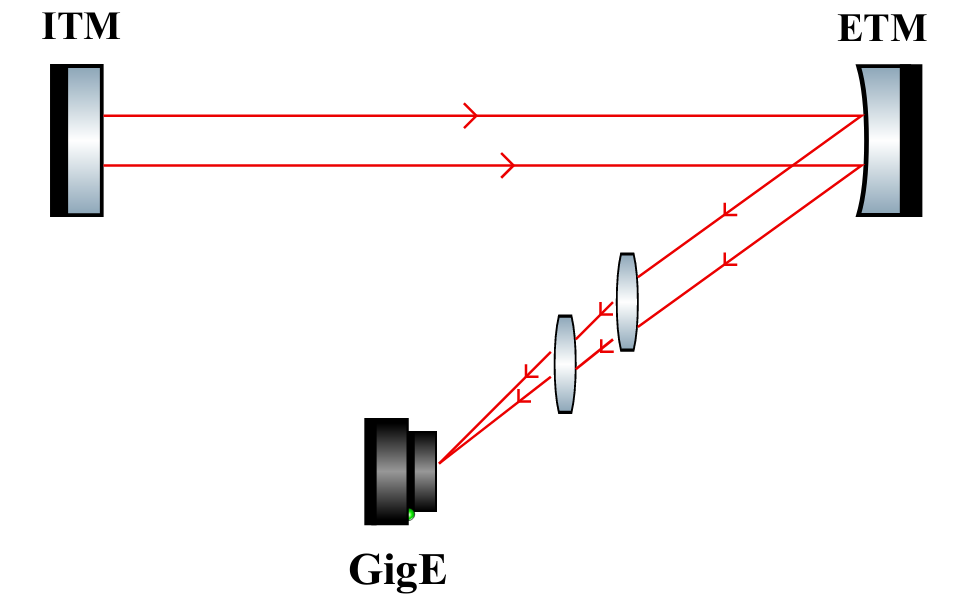
\includegraphics[width=.8\linewidth]{gige.png}
\caption{A schematic of a Fabry Perot cavity}
\label{fig:gige}
\end{center}
\end{figure} 


A typical control loop employing feedback control is illustrated in Figure \ref{fig:control_loop_bd}. Here, the dynamic system or the plant is an electronic or mechanical component whose output needs to be monitored and made to match the input reference. The plant could for instance be suspended optical components such as mirrors whose pitch and yaw eigenmodes need to be damped. The feedback sensor is used to monitor the behaviour of plant and provide the information necessary to produce the desired control signal to the controller. In the case of the optical lever system used for angular control, the working of which is elucidated in greater detail in Section \ref{objectives}, this is a quadrant photodetector that tracks the position of the reflected laser beam. 


\begin{figure}[htbp]
\begin{center}
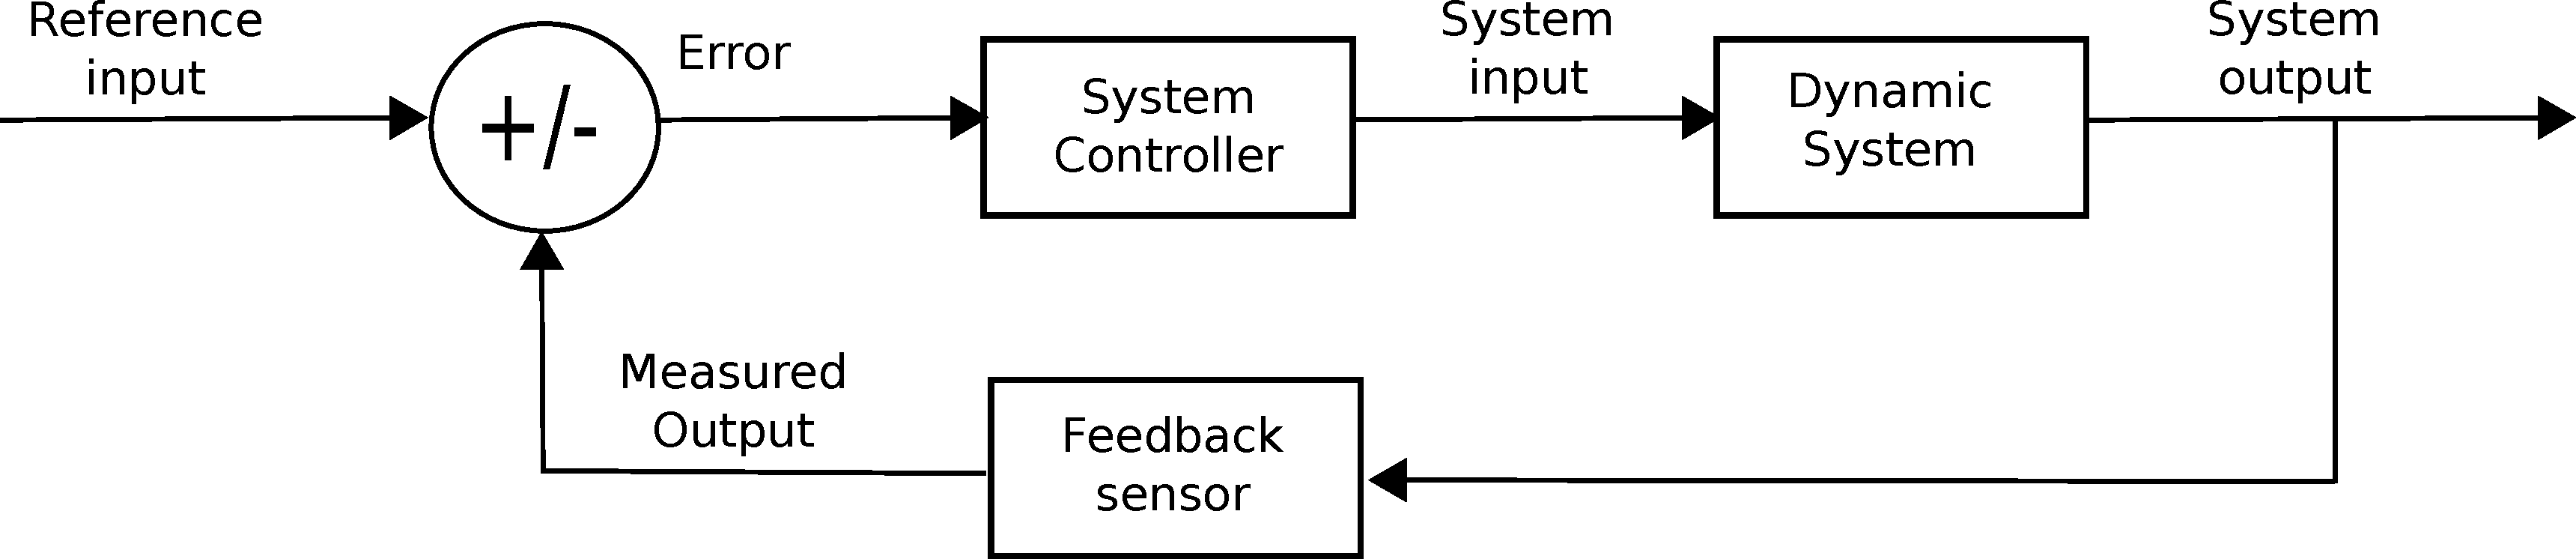
\includegraphics[width=.7\linewidth]{control_loop_bd.pdf}
\caption{A typical feedback control loop}
\label{fig:control_loop_bd}
\end{center}
\end{figure} 

A simple schematic of the sensing and control tasks is presented in Figure \ref{fig:overall}. 

\begin{figure}[htbp]
\begin{center}
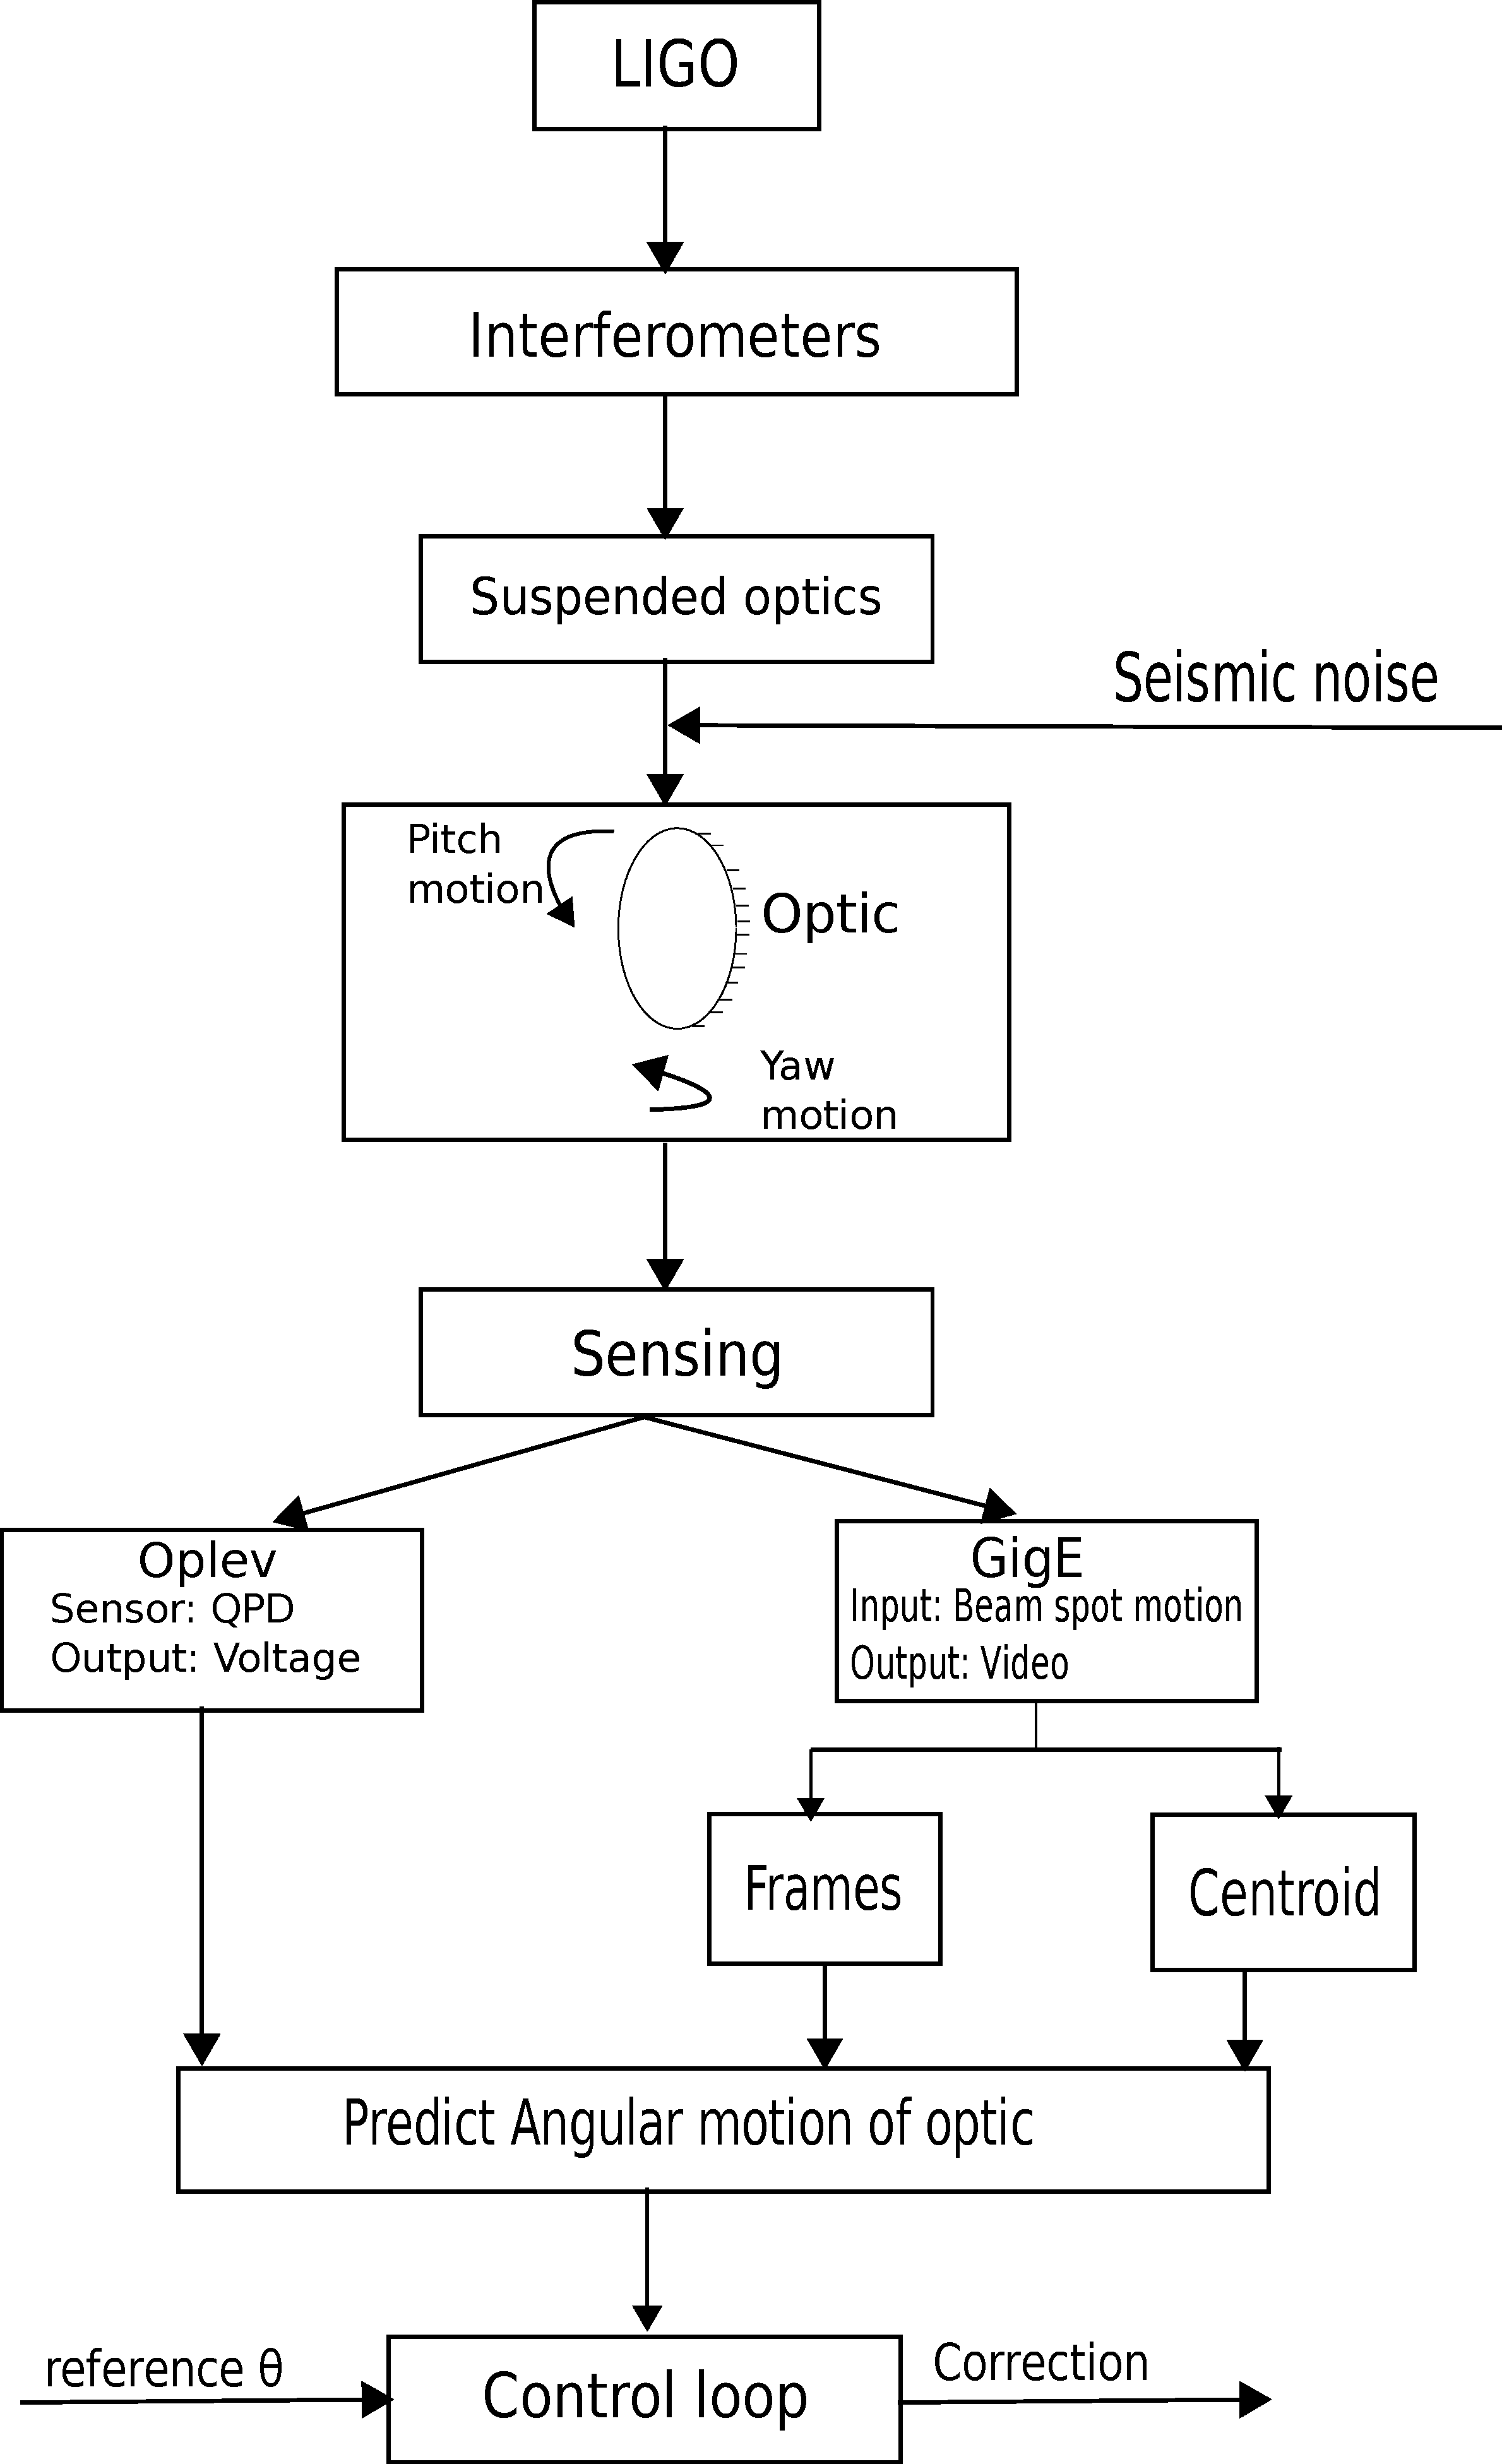
\includegraphics[width=.7\linewidth]{overall.pdf}
\caption{Sensing and control of angular motion}
\label{fig:overall}
\end{center}
\end{figure} 

Feedback control such as this is used to ensure that the LIGO interferometers remain in the observing mode despite being subject to numerous disturbances. Further, in an ideal case, the plant and the sensor are both linear i.e their output is proportional to their input and consequently, no feedback control is necessary. However, most real systems display a degree of non-linearity which is not desirable. Feedback control is used to ensure that the system operates in the linear region. An alternative is to use feedforward control and this has been employed successfully LIGO for instance in \cite{feedforward}. However, this requires very precise mathematical modelling of the system and is hard to do. As was observed in \cite{feedforward}, it is quite possible that the characterization of the system changes with time and this requires that the transfer functions be remeasured in a time consuming process in order to obtain optimal performance. Feedback control, on the other hand, is adaptive and therefore, more attractive. 


Most feedback techniques employed thus far rely on linear control to achieve the desired performance. However, most subsystems inevitably display non-linear and time dependent behaviour. Thus linear modeling is only an approximation of the behaviour of these subsystems for certain ranges of values. Further, the sensors used to monitor the plant themselves provide linear response when operated in certain regions. This has been explained in greater detail in Section 
\ref{objectives} in the context of the quadrant photodiode used in optical levers. Non-linear control schemes offer us the ability to model such responses and incorporate them into feedback for greater operating regions with fewer constraints. Further, when feedback signals are modeled as outputs of neural networks, they are computationally efficient during test time. Therefore, this work will attempt to explore the use of non-linear control to stabilise the aforementioned control loops and thus determine its applicability and efficacy at doing the same. This work will also attempt to borrow techniques from the rapidly advancing area of deep learning for the purpose of system identification and stabilization.   





% If you need to cite a source, do it like this: \cite{CitationKeyWord}.

% Pictures and figures are awesome!  You should include them wherever
% they will help make something more clear, as you can see in Figure \ref{fig:FigureKeyWord}.

%  \begin{figure}[htbp]
% \begin{center}
% \includegraphics[width=6in]{LIGOX_29March2011.jpg}
% \caption{LIGOX - The LIGO Instrument Science Group at Caltech.}
% \label{fig:FigureKeyWord}
% \end{center}
% \end{figure}         



\section{Objectives}\label{objectives}

    Irregularities on the surface and angular deviations of the suspended optics cause scattering which reduces optical power generated in the cavities and can lead to loss of lock. Ideally, a laser beam incident normally on a reflecting surface should not produce a beam spot visible to an observer at an angle. However, deviation of the light beam produces a beam spot on the camera (as shown in Figure \ref{fig:gige}). The test mass and the beam spot are brought to focus using a combination of two biconvex lenses. This setup allows one to monitor the motion of the optic by observing the motion of the beam spot. The properties of the beam spot such as the intensity and motion depend on the scattering the point of observation. The relation between the motion of the beam spot and the angular motion of the mirror can be determined theoretically. However, a neural network can also be used to capture this relationship when using real data. In this work, emphasis will be laid on developing robust algorithms for beam tracking with a general outline being highlighted in Section \ref{approach}.
   

% \begin{itemize}
    Following the development of better algorithms for sensing, this work will focus on using the signals from the beam tracking project and the optical lever system described subsequently to develop control algorithms that help the interferometer lock faster and over wider parameter spaces.
    % While using non-linear control, particularly neural networks to provide feedback is appealing, it requires that we show that these proposed techniques possess the potential to outperform pre-existing algorithms. For this, we will use a standard problem such as the inverted pendulum on a cart as a benchmark and compare the performance of the hitherto used techniques with that of the proposed algorithms. The inverted pendulum on a cart is a particularly attractive toy problem as it possesses a rich body of literature and has been the subject of much study. While this shall not be the primary focus of this project which shall lay greater emphasis on problems with the prototype interferometer, it presents a degree of theoretical grounding for the use of deep learning techniques in feedback loops.%\G{This kind of toy example is a good idea I think, but once you are in the lab, I would spend time on problems we are dealing with w.r.t. the interferometer}

    


    % \G{Such a comparison also requires the identification of suitable metrics to judge the relative performance of the proposed algorithms. Thus, an important portion of the earlier body of work will be the identification of the appropriate metrics. What are some potential \textit{quantitative} metrics we can use? }
    

    %%%%%%%%%%%%%% What is the oplev? 

    The optical lever is a subsystem integral for the angular control of suspended optics. Optical levers are used for the restoration of alignment after loss of lock \cite{optlev_note}. Figure \ref{fig:oplev_schematic} depicts a simple optical lever consisting of a fiber coupled diode laser, optics necessary to control beam size, quad photodetectors to determine beam location and displacement and structural pylons to mount the necessary hardware. 

    \begin{figure}[htbp]
    \begin{center}
    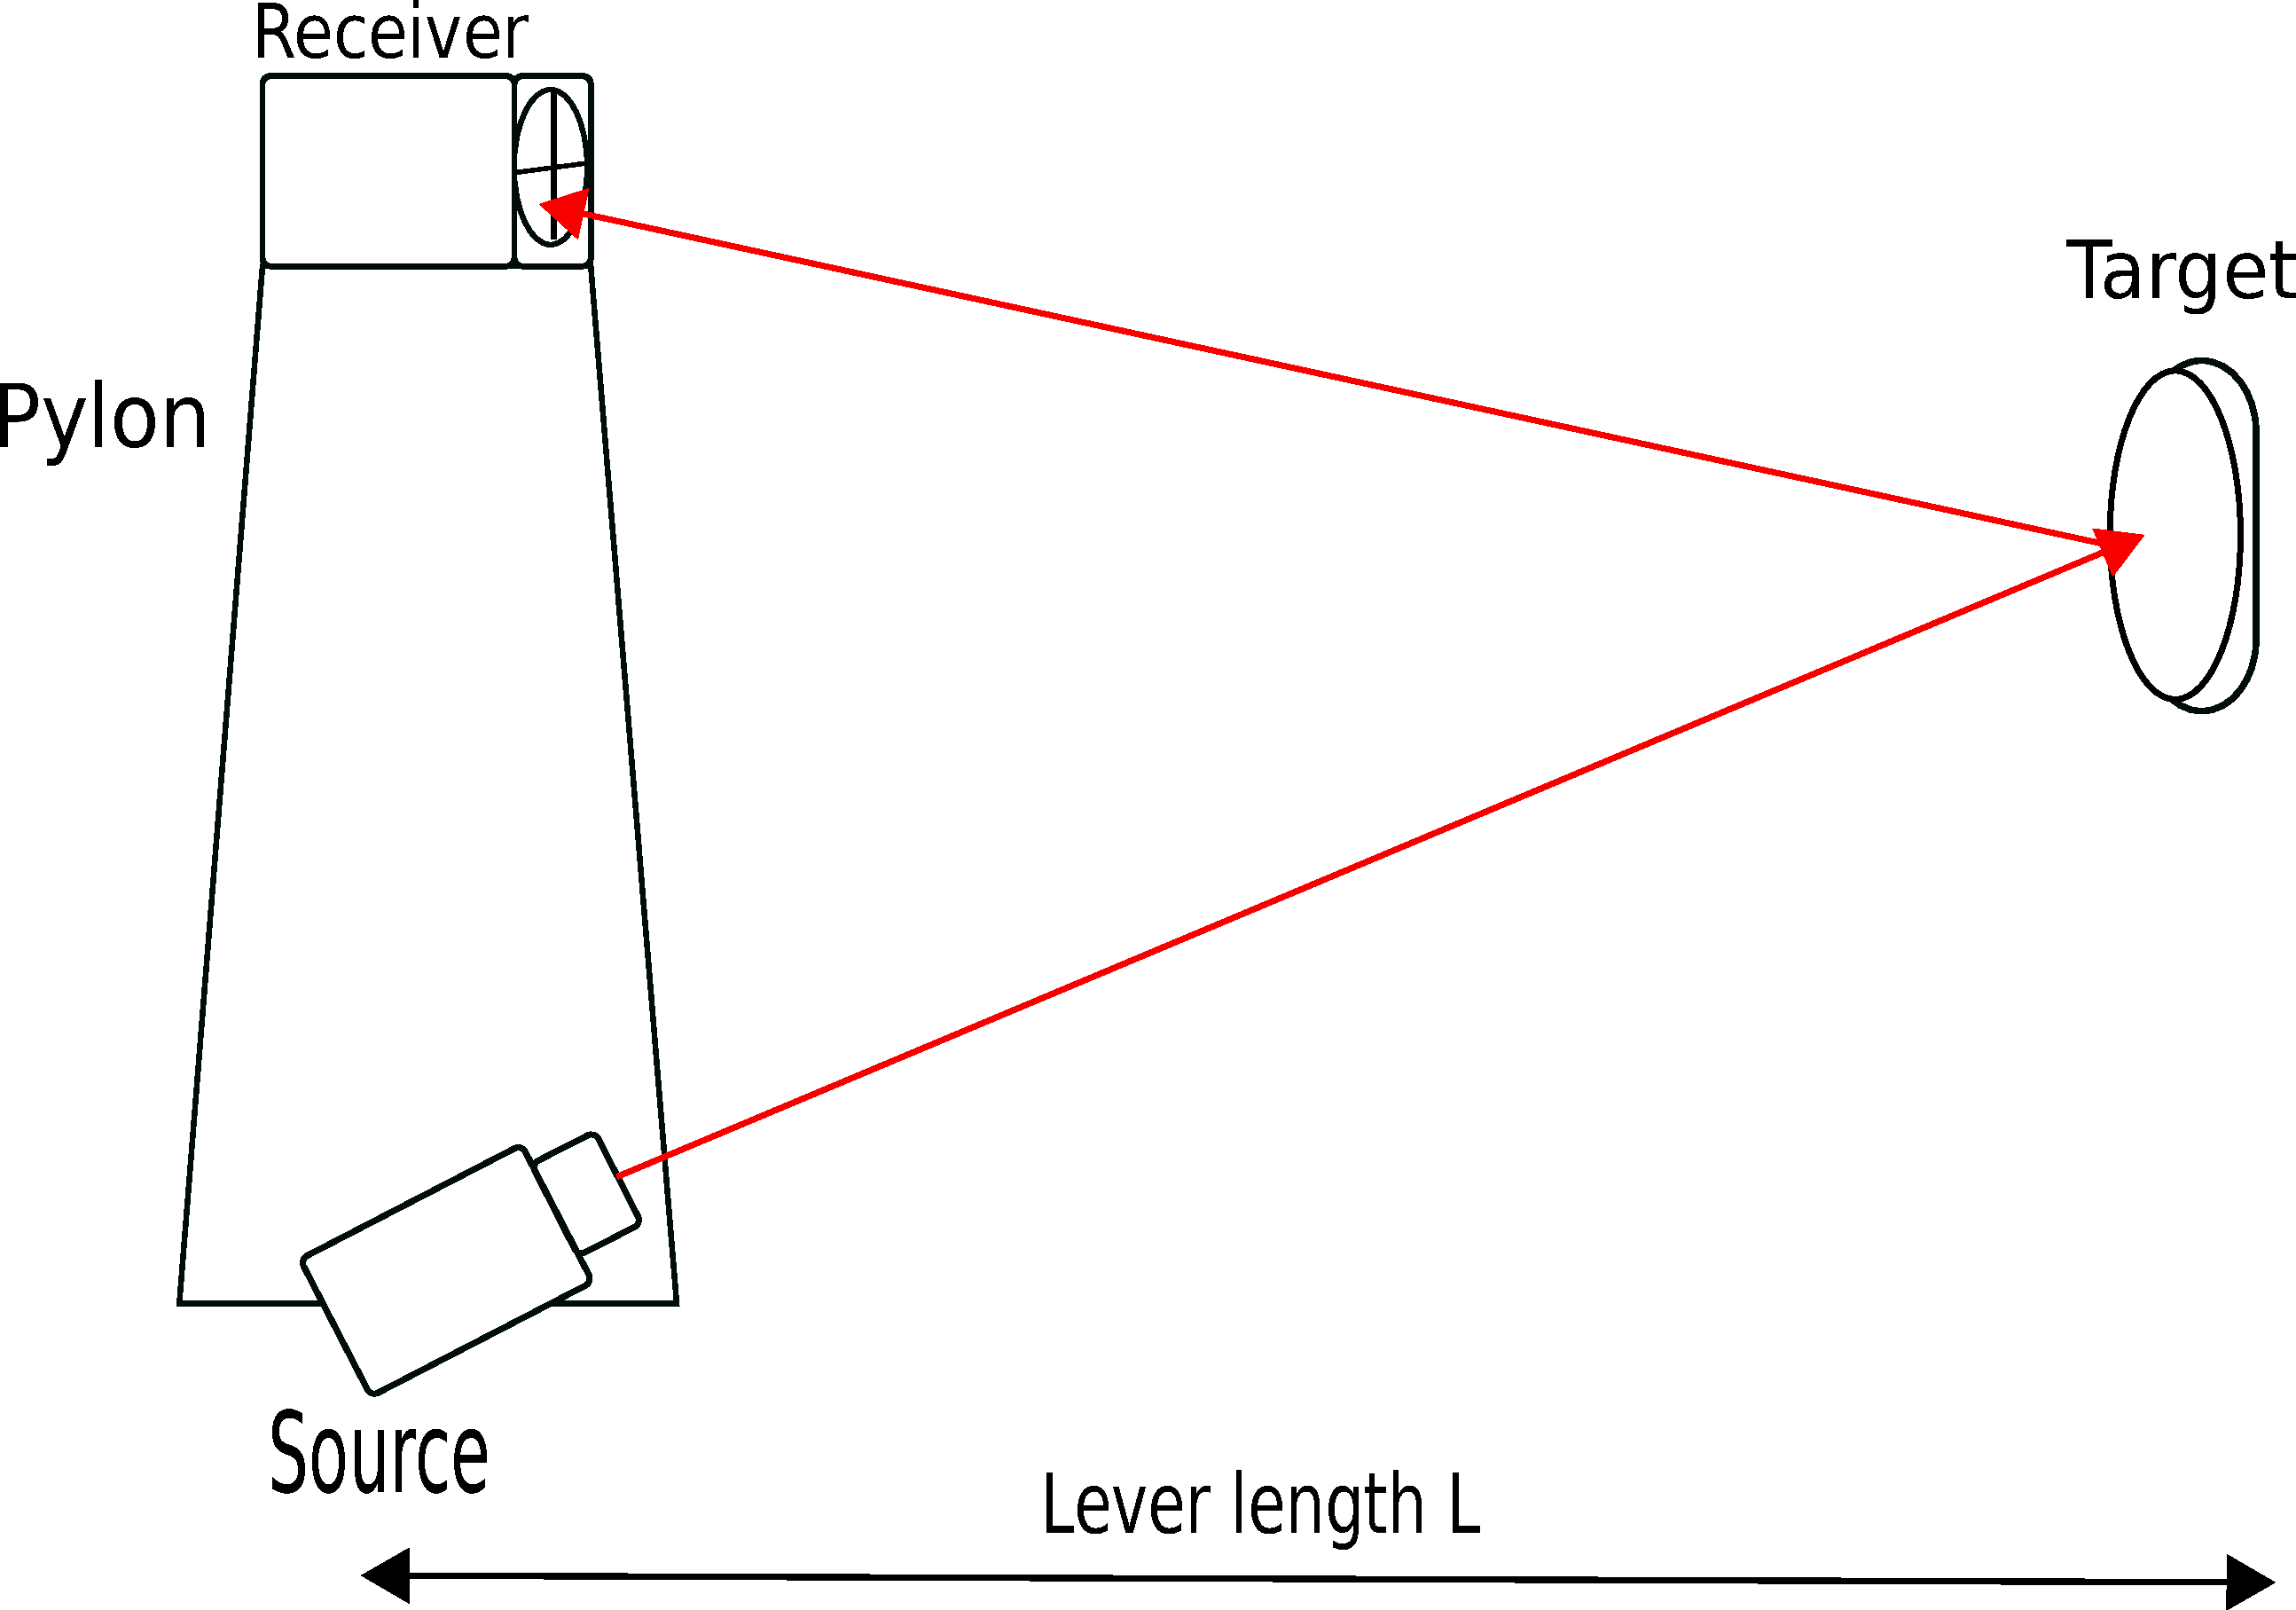
\includegraphics[width =.7\linewidth]{oplev_schematic.pdf}
    \caption{Design of an optical lever}
    \label{fig:oplev_schematic}
    \end{center}
    \end{figure} 

    The optical lever system helps stabilise the suspended mirrors to seismic noise. This is done by projecting a laser beam onto the suspended mirror and structuring the system to obtain the reflected beam on the quad photodetector. The system is calibrated such that the beam is centered perfectly when the mirrors are aligned. However, if the suspended mirror rotates through an angle $\theta$, then the reflected beam rotates through an angle $2\theta$. This is shown in Figure \ref{fig:2theta}. The position of the beam produces outputs say A, B, C, D (see Figure \ref{fig:qpd}) from the four quadrants which can be used to calculate the position of the beam using the following equations \cite{qpd_equations}

    \begin{align}
    x & = \frac{B + D - A - C}{A + B + C + D} \label{x}\\
    y & = \frac{A + B - C - D}{A + B + C + D} \label{y}
    \end{align}

    These signals are then used to provide feedback and align the mirrors suitably to obtain lock. However, the above relations are only approximate when the change in incident power is non-uniform across quadrants given a motion of the beam. Therefore, the use of a laser beam of circular cross section introduces some error in the measurement and limits the linear range. Further, laser beams have a Gaussian intensity profile which further limits the linear range. It is here that non-linear control can be used to improve the feedback mechanisms to achieve better modelling and performance.


    \begin{figure}[htbp]
      \centering
        \begin{subfigure}[b]{0.4\textwidth}
          \centering
          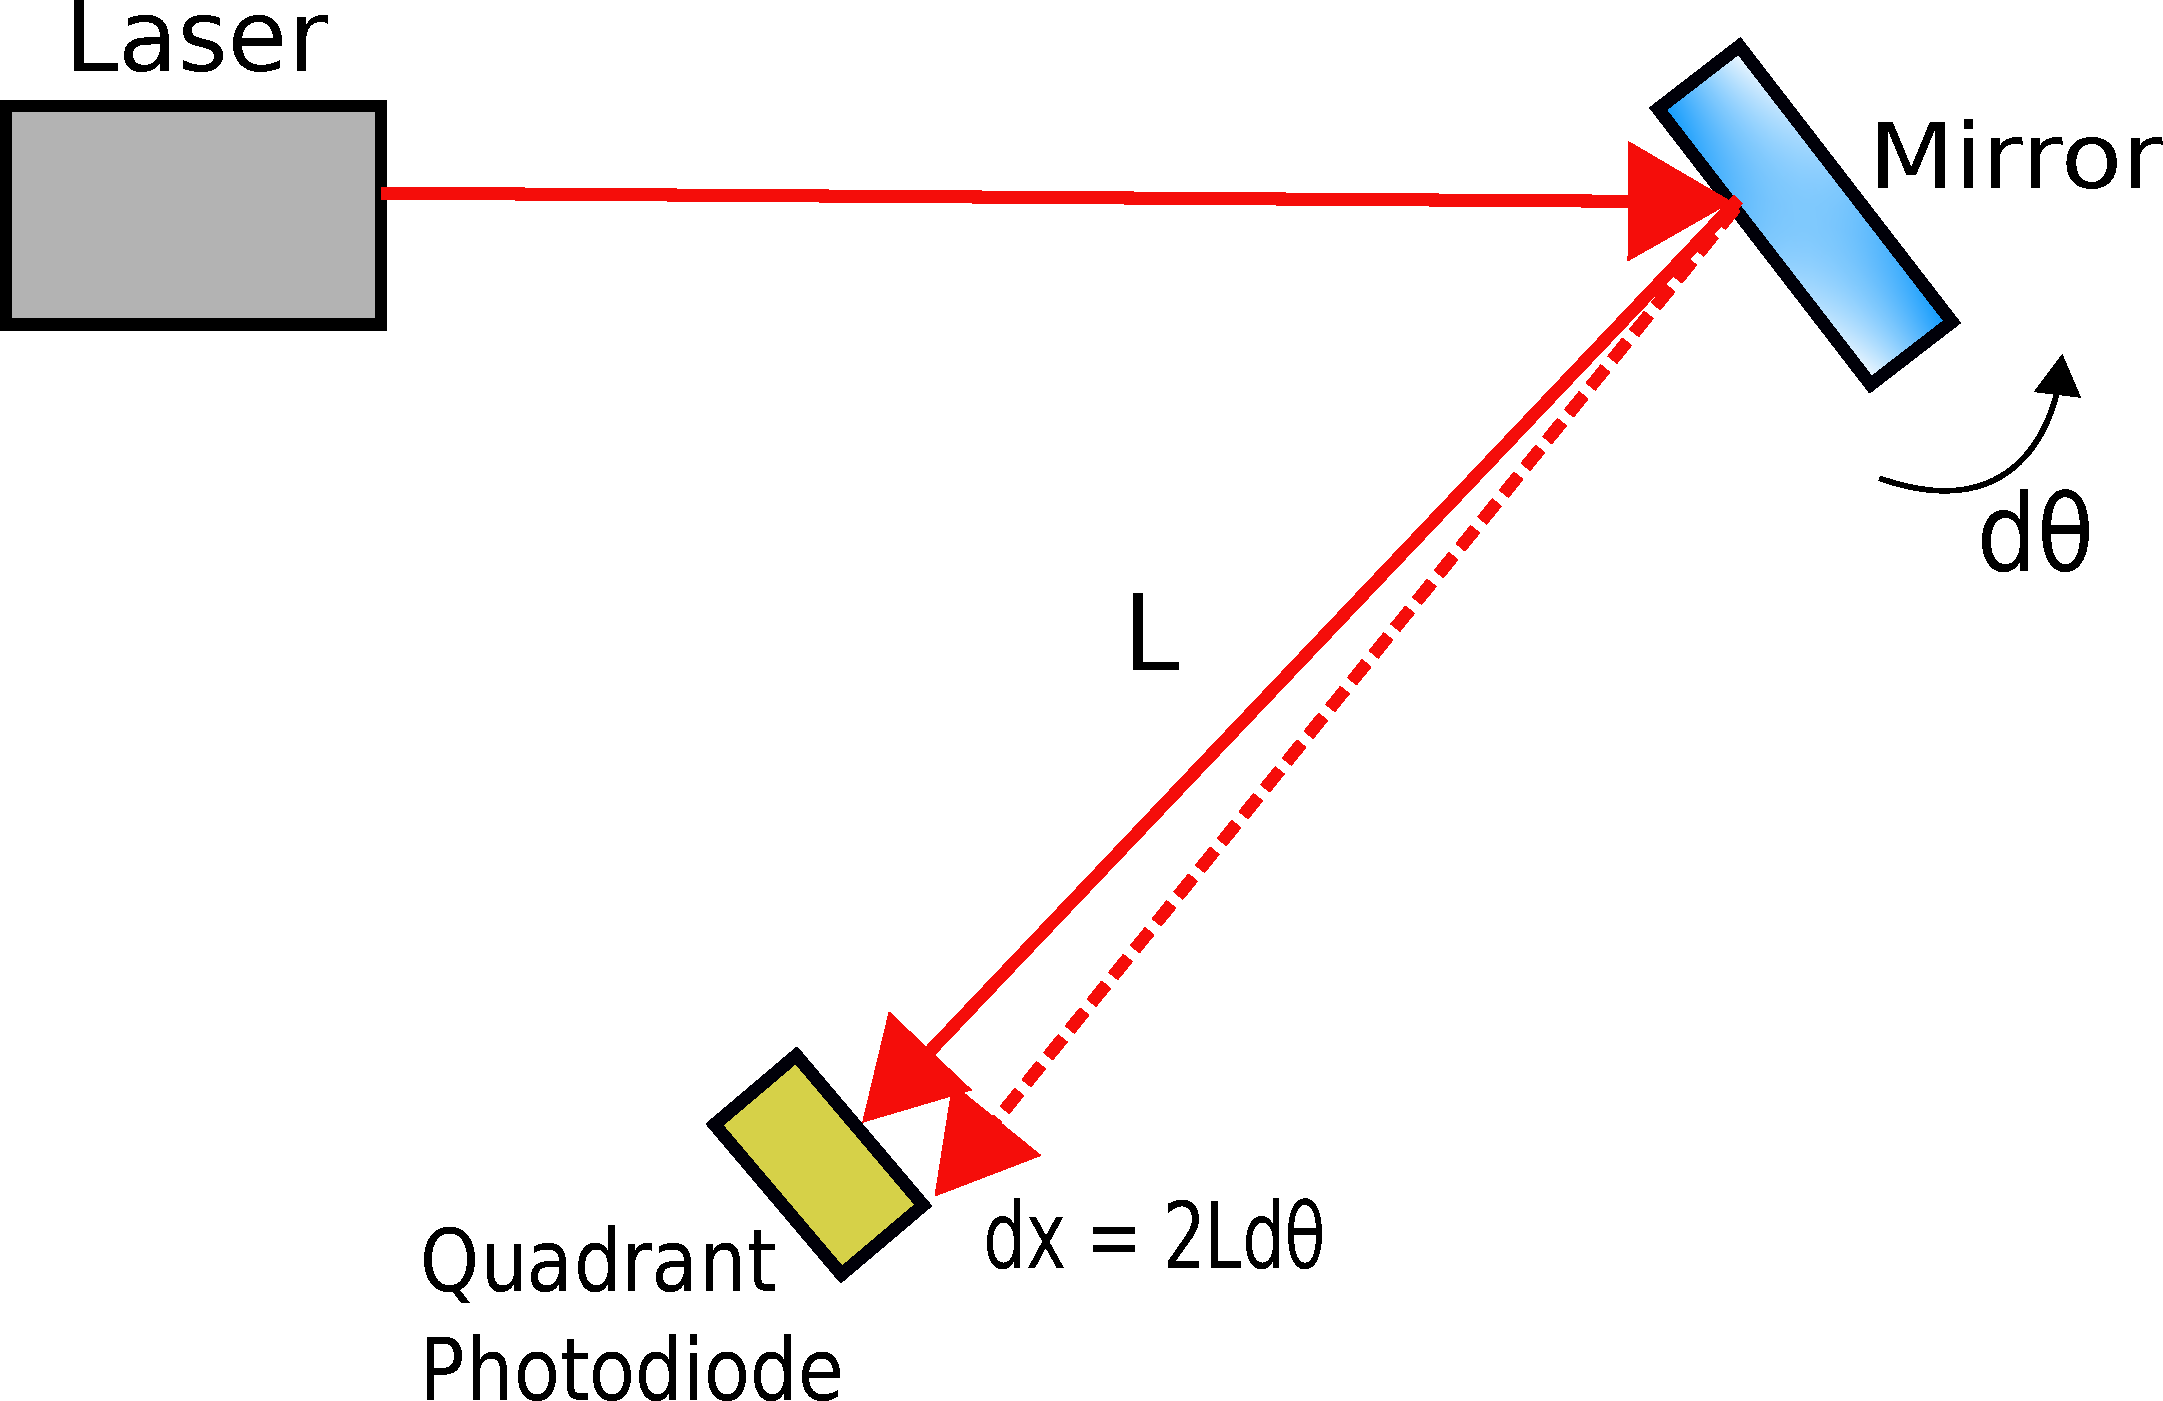
\includegraphics[width=\linewidth]{2theta.pdf}
          \caption{}
          \label{fig:2theta}
        \end{subfigure}%
        \begin{subfigure}[b]{0.4\textwidth}
          \centering
          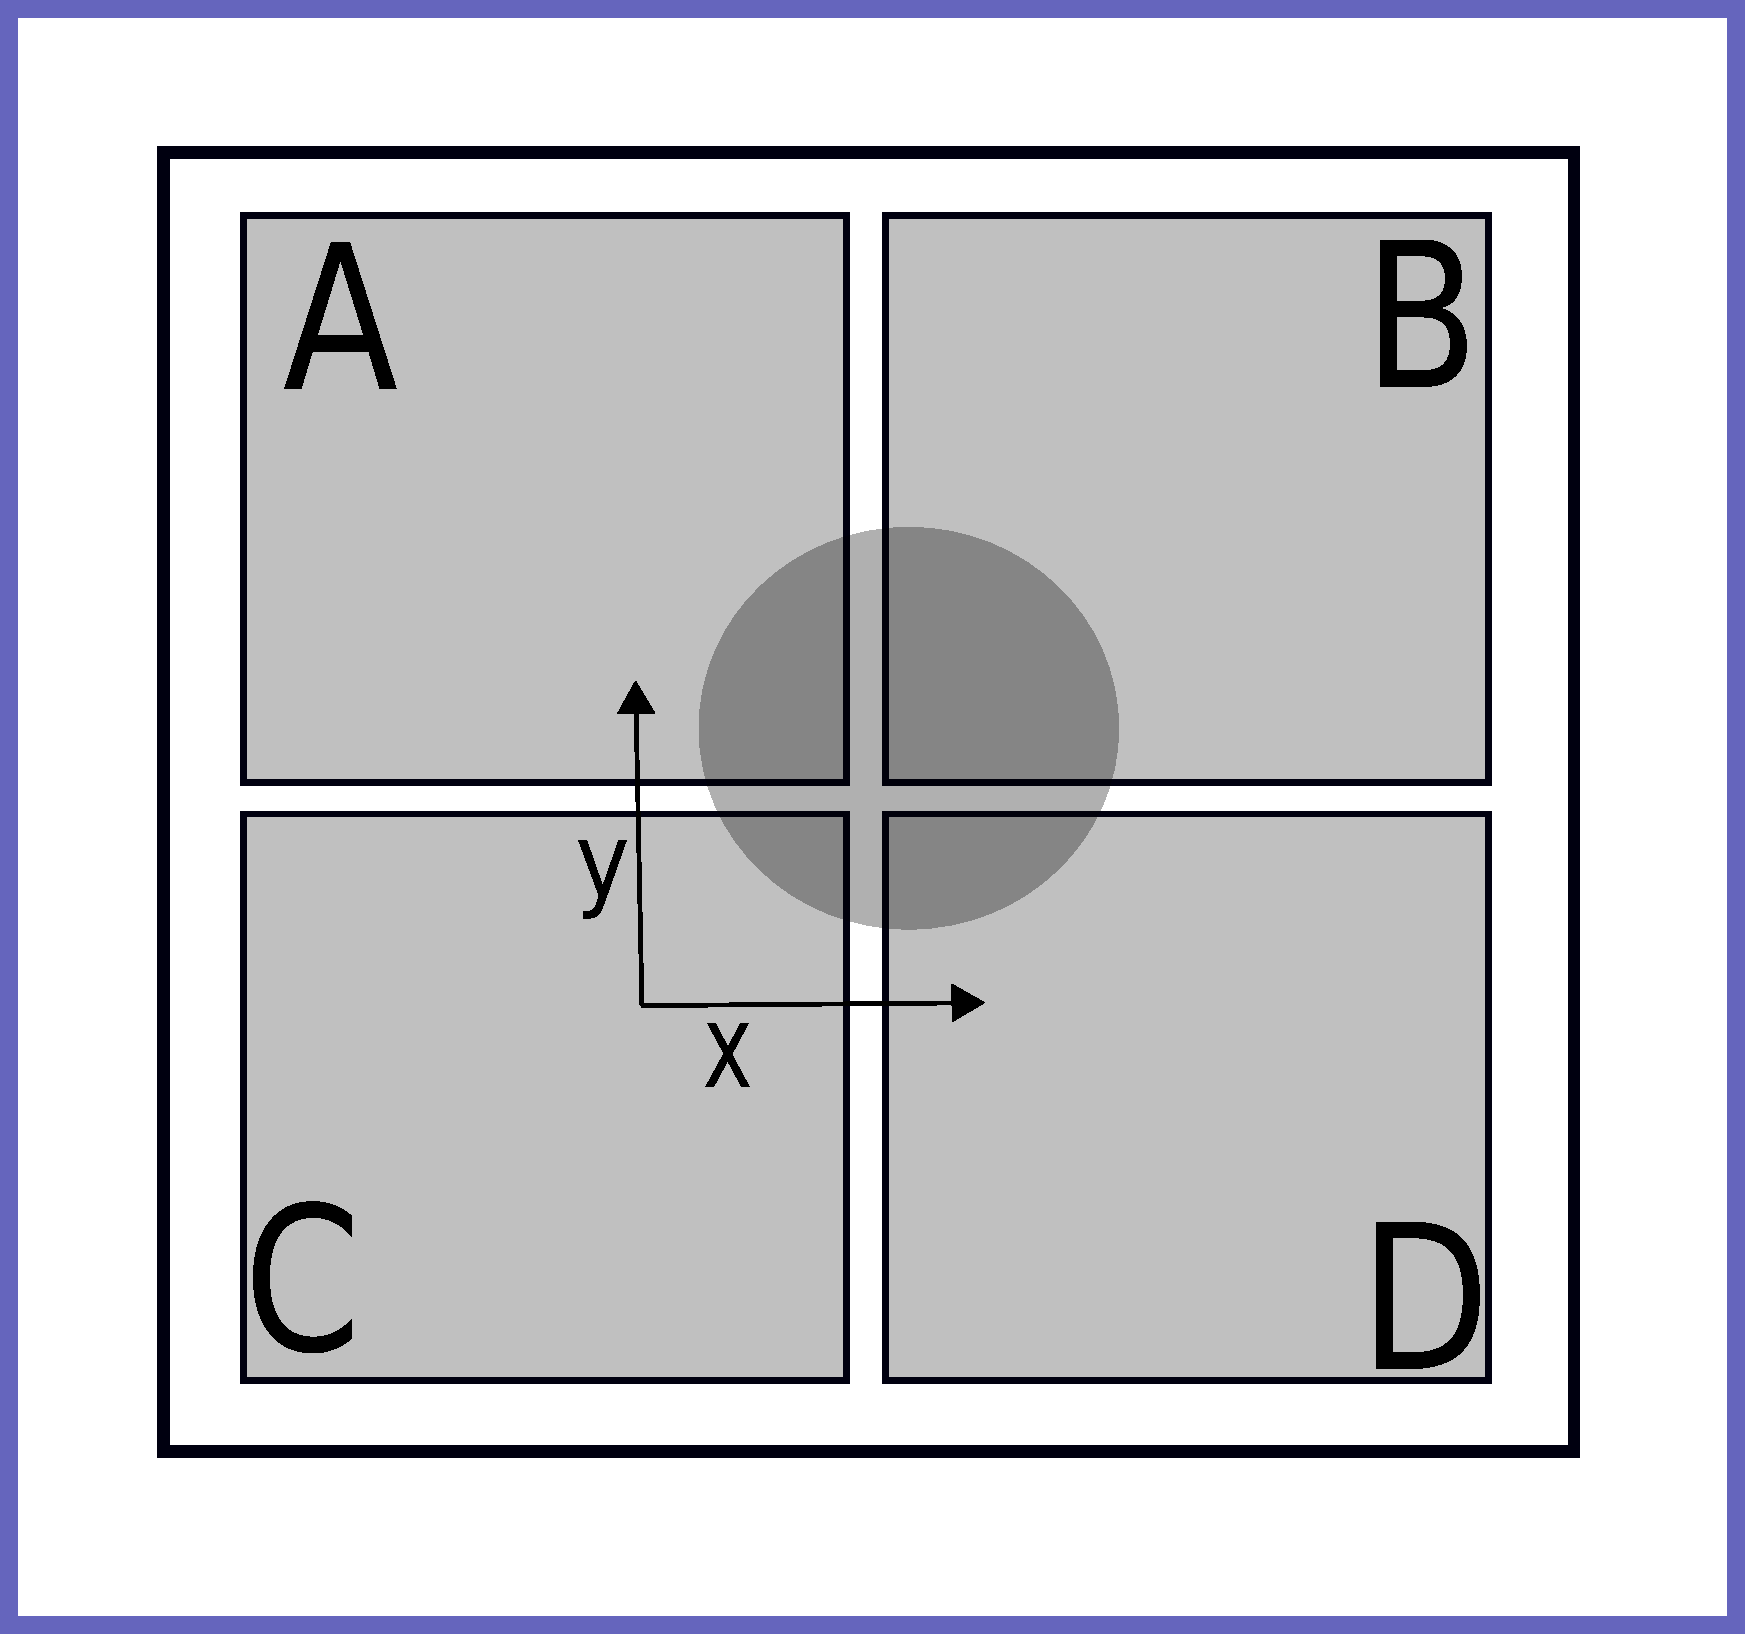
\includegraphics[width=0.5\linewidth]{qpd.pdf}
          \caption{}
          \label{fig:qpd}
        \end{subfigure}
      \caption{Simplified representations of the optical lever system (a) Angular deflection of the mirror and reflected beam \cite{control_slides} (b) Illustration of a four quandrant photodiode}
      \label{fig:oplev}
    \end{figure}     


    % \G{This will actually be the main project, so we should expand on this. What exactly is the beam tracking project? Some diagrams will be useful.} 

    Another control scheme worth considering is feedforward control which requires complete knowledge of the system to design filters that perform the necessary actions. As mentioned in Section \ref{introduction}, this is not adaptive and performance can decrease with time as the coupling of noise and the system model change. However, this does have the advantage of being unconditionally stable which is a major advantage over feedback control loops that need to be carefully designed to not become unstable. This is of great significance considering the fact that even the slightest error in alignment or calibration of optical components can lead to one control loop injecting noise into another control loop or driving it to instability. Optical components such as mirrors used in optical cavities are suspended to isolate them from seismic noise. However, this leads to translational ground motion being converted to angular motion due to the design of the seismic isolation systems \cite{feedforward}. This essentially implies a time varying model for the suspended mirrors. Consequently, feedforward control does not immediately appear to be a promising option for the control of such a system. However, a more careful investigation of its feasilbilty will be carried out before it is dismissed out of hand.



% \end{itemize}

\section{Approach}\label{approach}
    
    The first step will be to set up a simple simulation of a circular beam spot with intensity varying as a Gaussian that moves about along one axis. Python code shall be written to detect the centroid of the beam. Initial attempts shall involve using standard computer vision algorithms. Neural network based methods need to be employed to determine the angular motion of the optic. In that case, the input data to the neural network will consist of frames of the video. In the case of feedforward networks, this would translate to preprocessed framewise data. In the case of convolutional neural networks, the frames can be used as is to output a value. In all these cases, the output is a real value and thus a loss function such as mean square error can be used to measure the performance of the network. A schematic is presented in Figure \ref{fig:train}.

    \begin{figure}[htbp]
    \begin{center}
    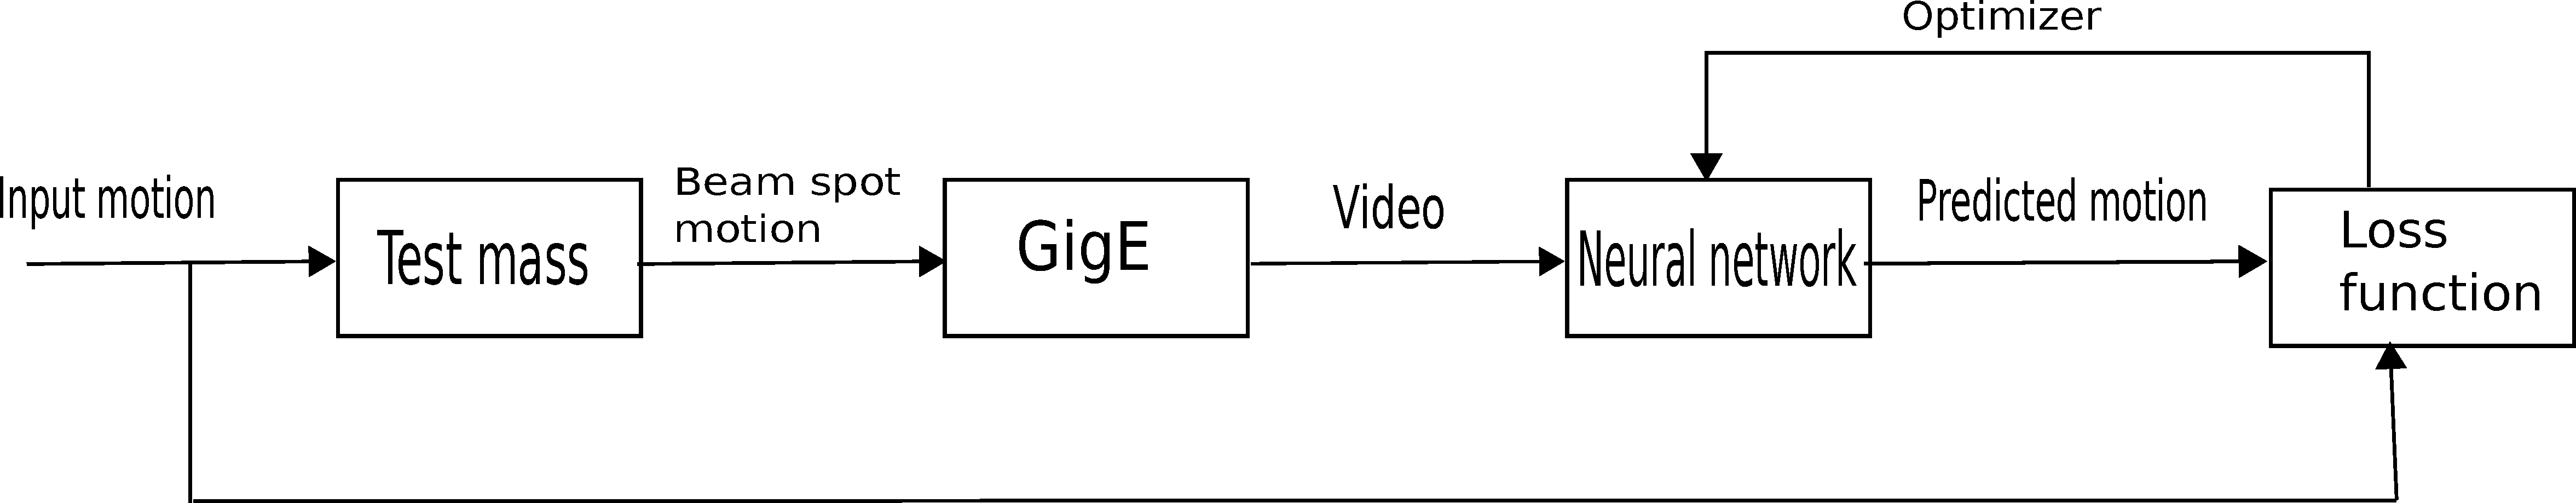
\includegraphics[width =.7\linewidth]{train.pdf}
    \caption{Training a neural network to determine angular motion}
    \label{fig:train}
    \end{center}
    \end{figure}
    
    At test time input from the GigE will be used to predict the angular motion as in Figure \ref{fig:test}. Much of the experimentation will lie in tuning hyperparameters and determining the precise architecture to use. This setup works under the assumption that the GigE camera measures only the effects of angular motion. However, this is not true as the effects of scattering due to surface irregularities and other sources of noise too contribute to beam motion. Thus, a method needs to be devised to identify and isolate these effects from that of angular motion of the mirror. 

     In the case of the QPD, signal processing algorithms need to be applied to the outputs corresponding to the four quadrants of the photodiode to determine the position of the beam spot which in turn can be used to determine the motion of the plant (optic). The position of the beam spot on the QPD can be found using equations \ref{x} and \ref{y}. The angular motion of the optic can be computed theoretically by studying the setup of hardware. One important consideration here is the linear range of the QPD which will be evaluated through the collection and analysis of the QPD data. 

    \begin{figure}[htbp]
    \begin{center}
    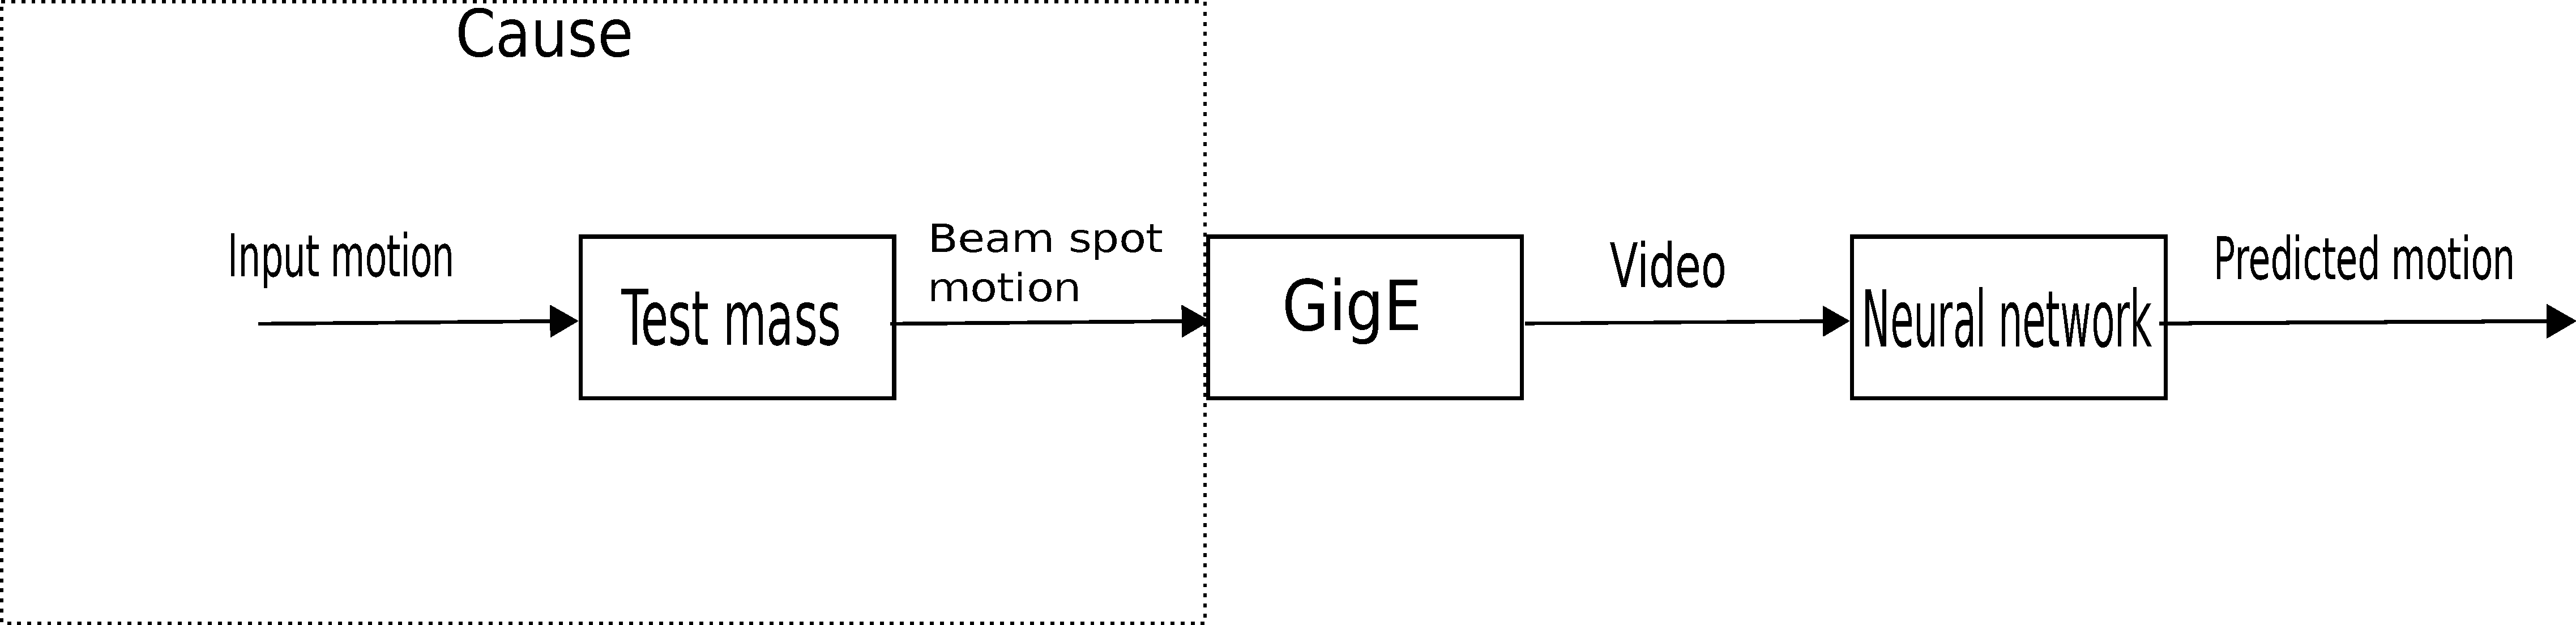
\includegraphics[width =.7\linewidth]{test.pdf}
    \caption{Neural network at test time}
    \label{fig:test}
    \end{center}
    \end{figure}  

    Once the motion of the plant is determined from the motion of the beam from either the camera or the QPD sensor, feedback control can be used to guide the mirror back into alignment to obtain lock and keep the interferometer in detection mode.
     
    %\G{Again, the last two bullets will be the main project. So let's have a block diagram/flowchart of the training process, validation, testing etc.} - done.

    % Once a subsystem is identified, the first step involved is system identification. This is depicted in Figure \ref{fig:plant_identification}. This is a crucial step of the process and determines the quality of the feedback control system. If the selected subsystem is the optical lever, then the plant is the suspended mirror. The motion of the mirror serves as the input and can be detected by the QPD output as discussed in Section \ref{objectives}. The network is expected to produce the same output as the mirror, measured as perhaps angular deviation, and is trained by minimizing the error between the predicted output and actual output of the plant. Since angular deviation is a continuous value, using a standard loss function like mean squared error will likely produce good results. The universal approximation theorem guarantees that the neural network will be able to model the plant over its entire operating range given that we use a sufficiently deep network.
    
    % \begin{figure}[htbp]
    % \begin{center}
    % \includegraphics[width =.7\linewidth]{plant_identification.png}
    % \caption{Plant identification using a neural network \cite{nncontrol}}
    % \label{fig:plant_identification}
    % \end{center}
    % \end{figure} 

    % Once such a non-linear model is obtained, the predictive control model based on the receding horizon technique described in \cite{nncontrol} can be used for the angular control of the suspended optics. 


    % In the case of laser beam tracking, both simulated and real data obtained from the cameras set up can be used to train the learning algorithms. The final step will be to implement these learning algorithms on the actual subsystem itself.

\section{Project Timeline}
\begin{itemize}
    \item Pre-arrival: Literature review of the use of neural networks in control engineering, control techniques already employed, subsystems of LIGO that non-linear control can possibly be applied to, code review of the previously written code on laser beam tracking
    \item Week 1: Continued literature review. Simulation of spot motion from previously written code.
    \item Week 2- 3: Tracking beam spot motion. Study of classical methods vs neural network based methods.
    \item Week 3 - 7: Identifying the control scheme to be used, acquiring and cleaning data, training the necessary models.
    \item Week 7 -11: Extending the developed algorithm to the actual subsystem. Report preparation and presentation.
\end{itemize}



\begin{thebibliography}{9}


  \bibitem{adhikari2004sensitivity}
    Rana Adhikari,
    \emph{Sensitivity and noise analysis of 4 km laser interferometric gravitational wave antennae}.
    PhD diss., Massachussetts Institute of Technology, 2004.

  \bibitem{feedforward}
    Ryan DeRosa, Jennifer C Driggers, Dani Atkinson, Haixing Miao, Valery Frolov, Michael Landry, JosephGiaime, Rana Adhikari. 
    \emph{Global Feed-Forward Vibration Isolation in a km scale Interferometer}.
    Class. Quantum Grav. 29 215008, 2012.

  \bibitem{optlev_note}
    Eric D. Black, Tara Chelermsongsak, Riccardo Desalvo,Zach Korth, Mark Barton, Doug Cook, 
    Cheryl Vorvick,Hiro Yamammoto, Giovanni Salvi, Rob Schofield, Michael Smith
    \emph{Advanced-LIGO Optical LeversDesign Requirements}.
    Internal working note, LIGO. 2010.
      
  % \bibitem{nncontrol}
  %   Martin T. Hagan, Howard B. Demuth, Orlando De Jesus
  %   \emph{An Introduction to the Use of Neural Networks in Control Systems}.
  %   Internal working note, LIGO.

    \bibitem{qpd_equations}
      \url{https://www.aptechnologies.co.uk/support/SiPDS/bicell-quad}

    \bibitem{control_slides}
      \url{https://dcc.ligo.org/public/0115/G1401146/002/Lecture_Control.pdf}

    \bibitem{gige}
      \url{https://dcc.ligo.org/public/0152/T1800245/002/final_report.pdf}


% 	\bibitem{CitationKeyWord}
% 	  Author,
% 	  \emph{Title of the Article or Book}.
% 	 Physical Review XXXX, XXXXX (2010).    
      
%       \bibitem{URLsource}
%       \url{http://blue.ligo-wa.caltech.edu:8000/40m/40mHomePage}
 
\end{thebibliography} %Must end the environment



\end{document} 
